\begin{frame}
\frametitle{Nasze rozwiązanie --- dla end-usera}

\begin{columns}[c]
	\begin{column}[t]{.45\textwidth}
		\vskip-5em
		\begin{enumerate}
			\item Android.
			\only<2->{\item Kompatybilność z programem XMind.}
			\only<3->{\item Kolaboracja online.}
			\only<4->{\item Synchronizacja offline.}
			\only<5->{\item Intuicyjny interfejs użytkownika.}
		\end{enumerate}
	\end{column}
	\begin{column}{.45\textwidth}
		\only<2->{\begin{figure}
			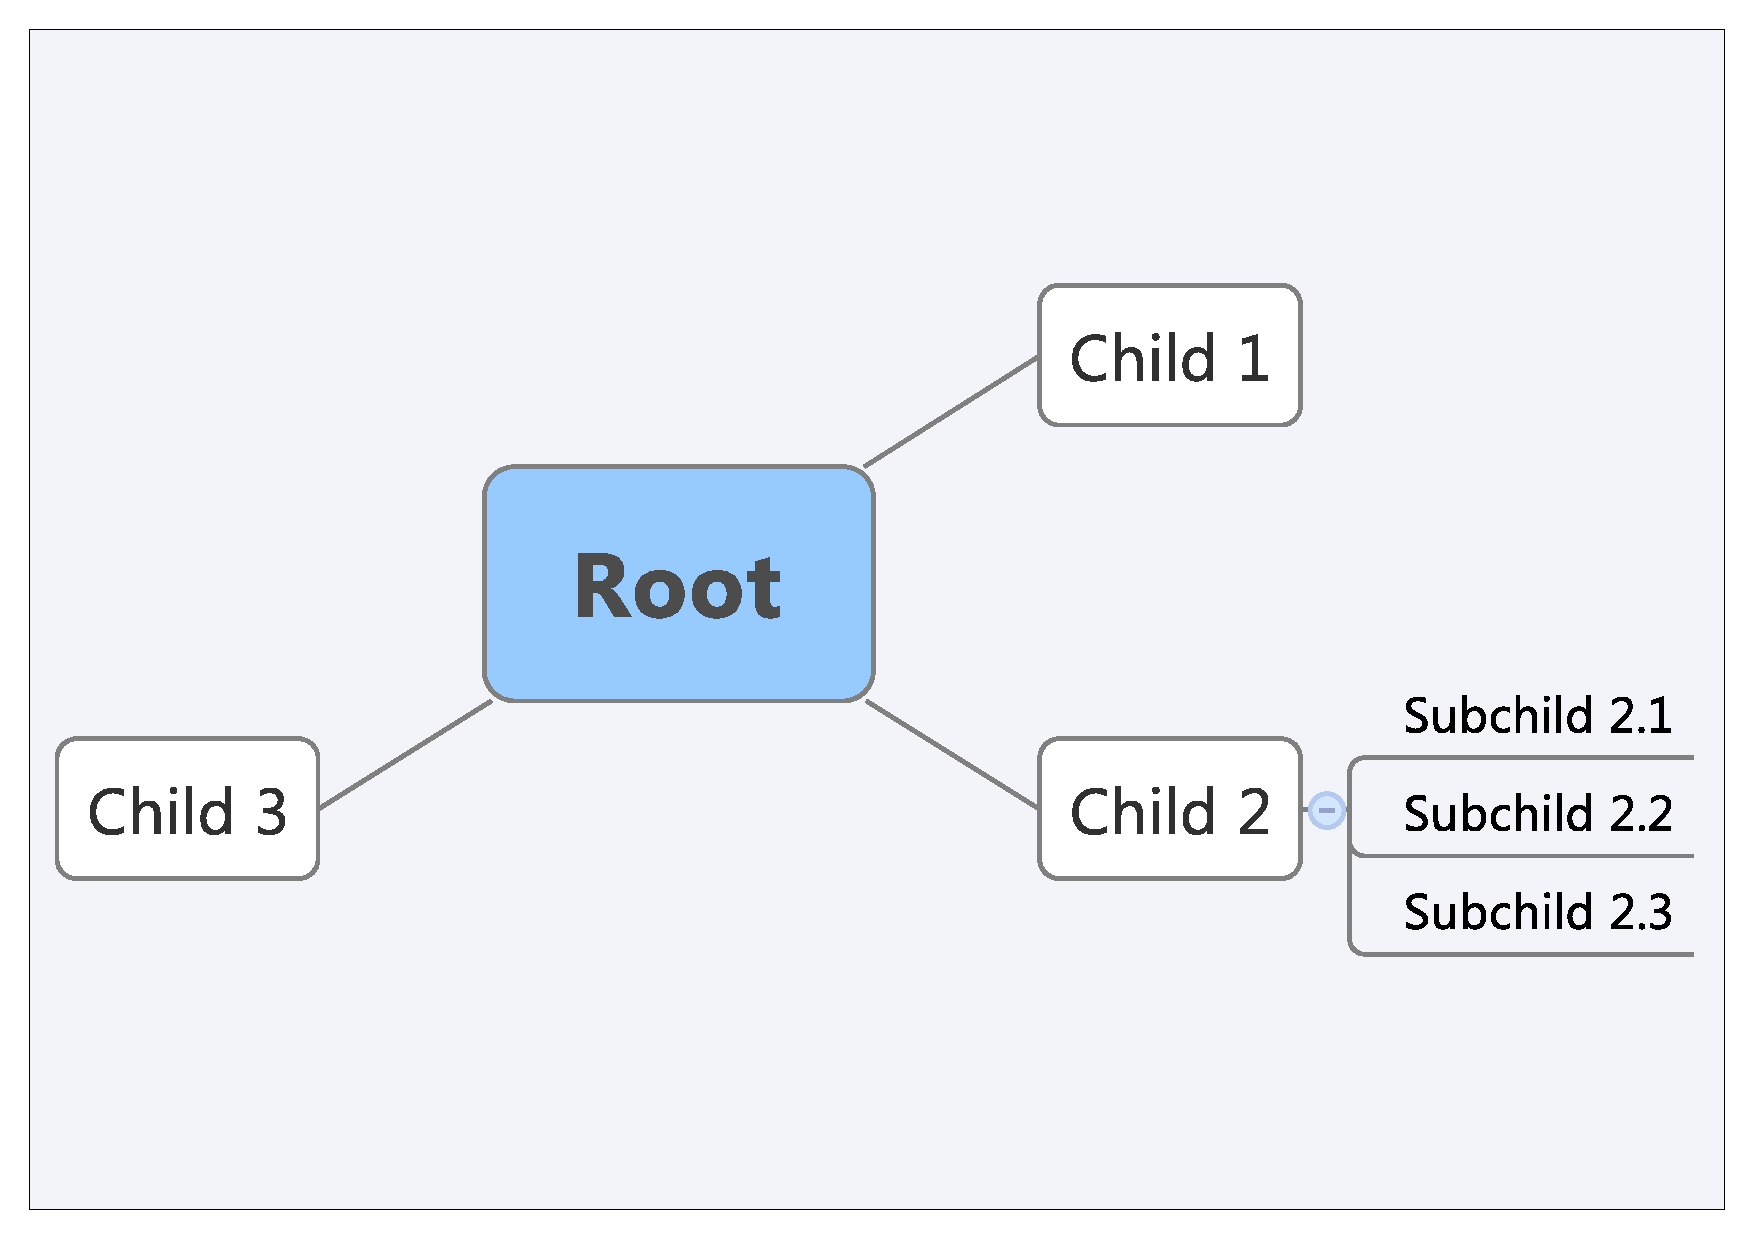
\includegraphics[width=\textwidth]{xmind}
			\caption{Mapa z programu XMind.}
		\end{figure}}
	\end{column}
\end{columns}

\end{frame}
